
\section{Results}

\subsection{Springs changing concentration with season, indicating monsoonal precipitation influence}

\begin{figure}[h]
    \centering
    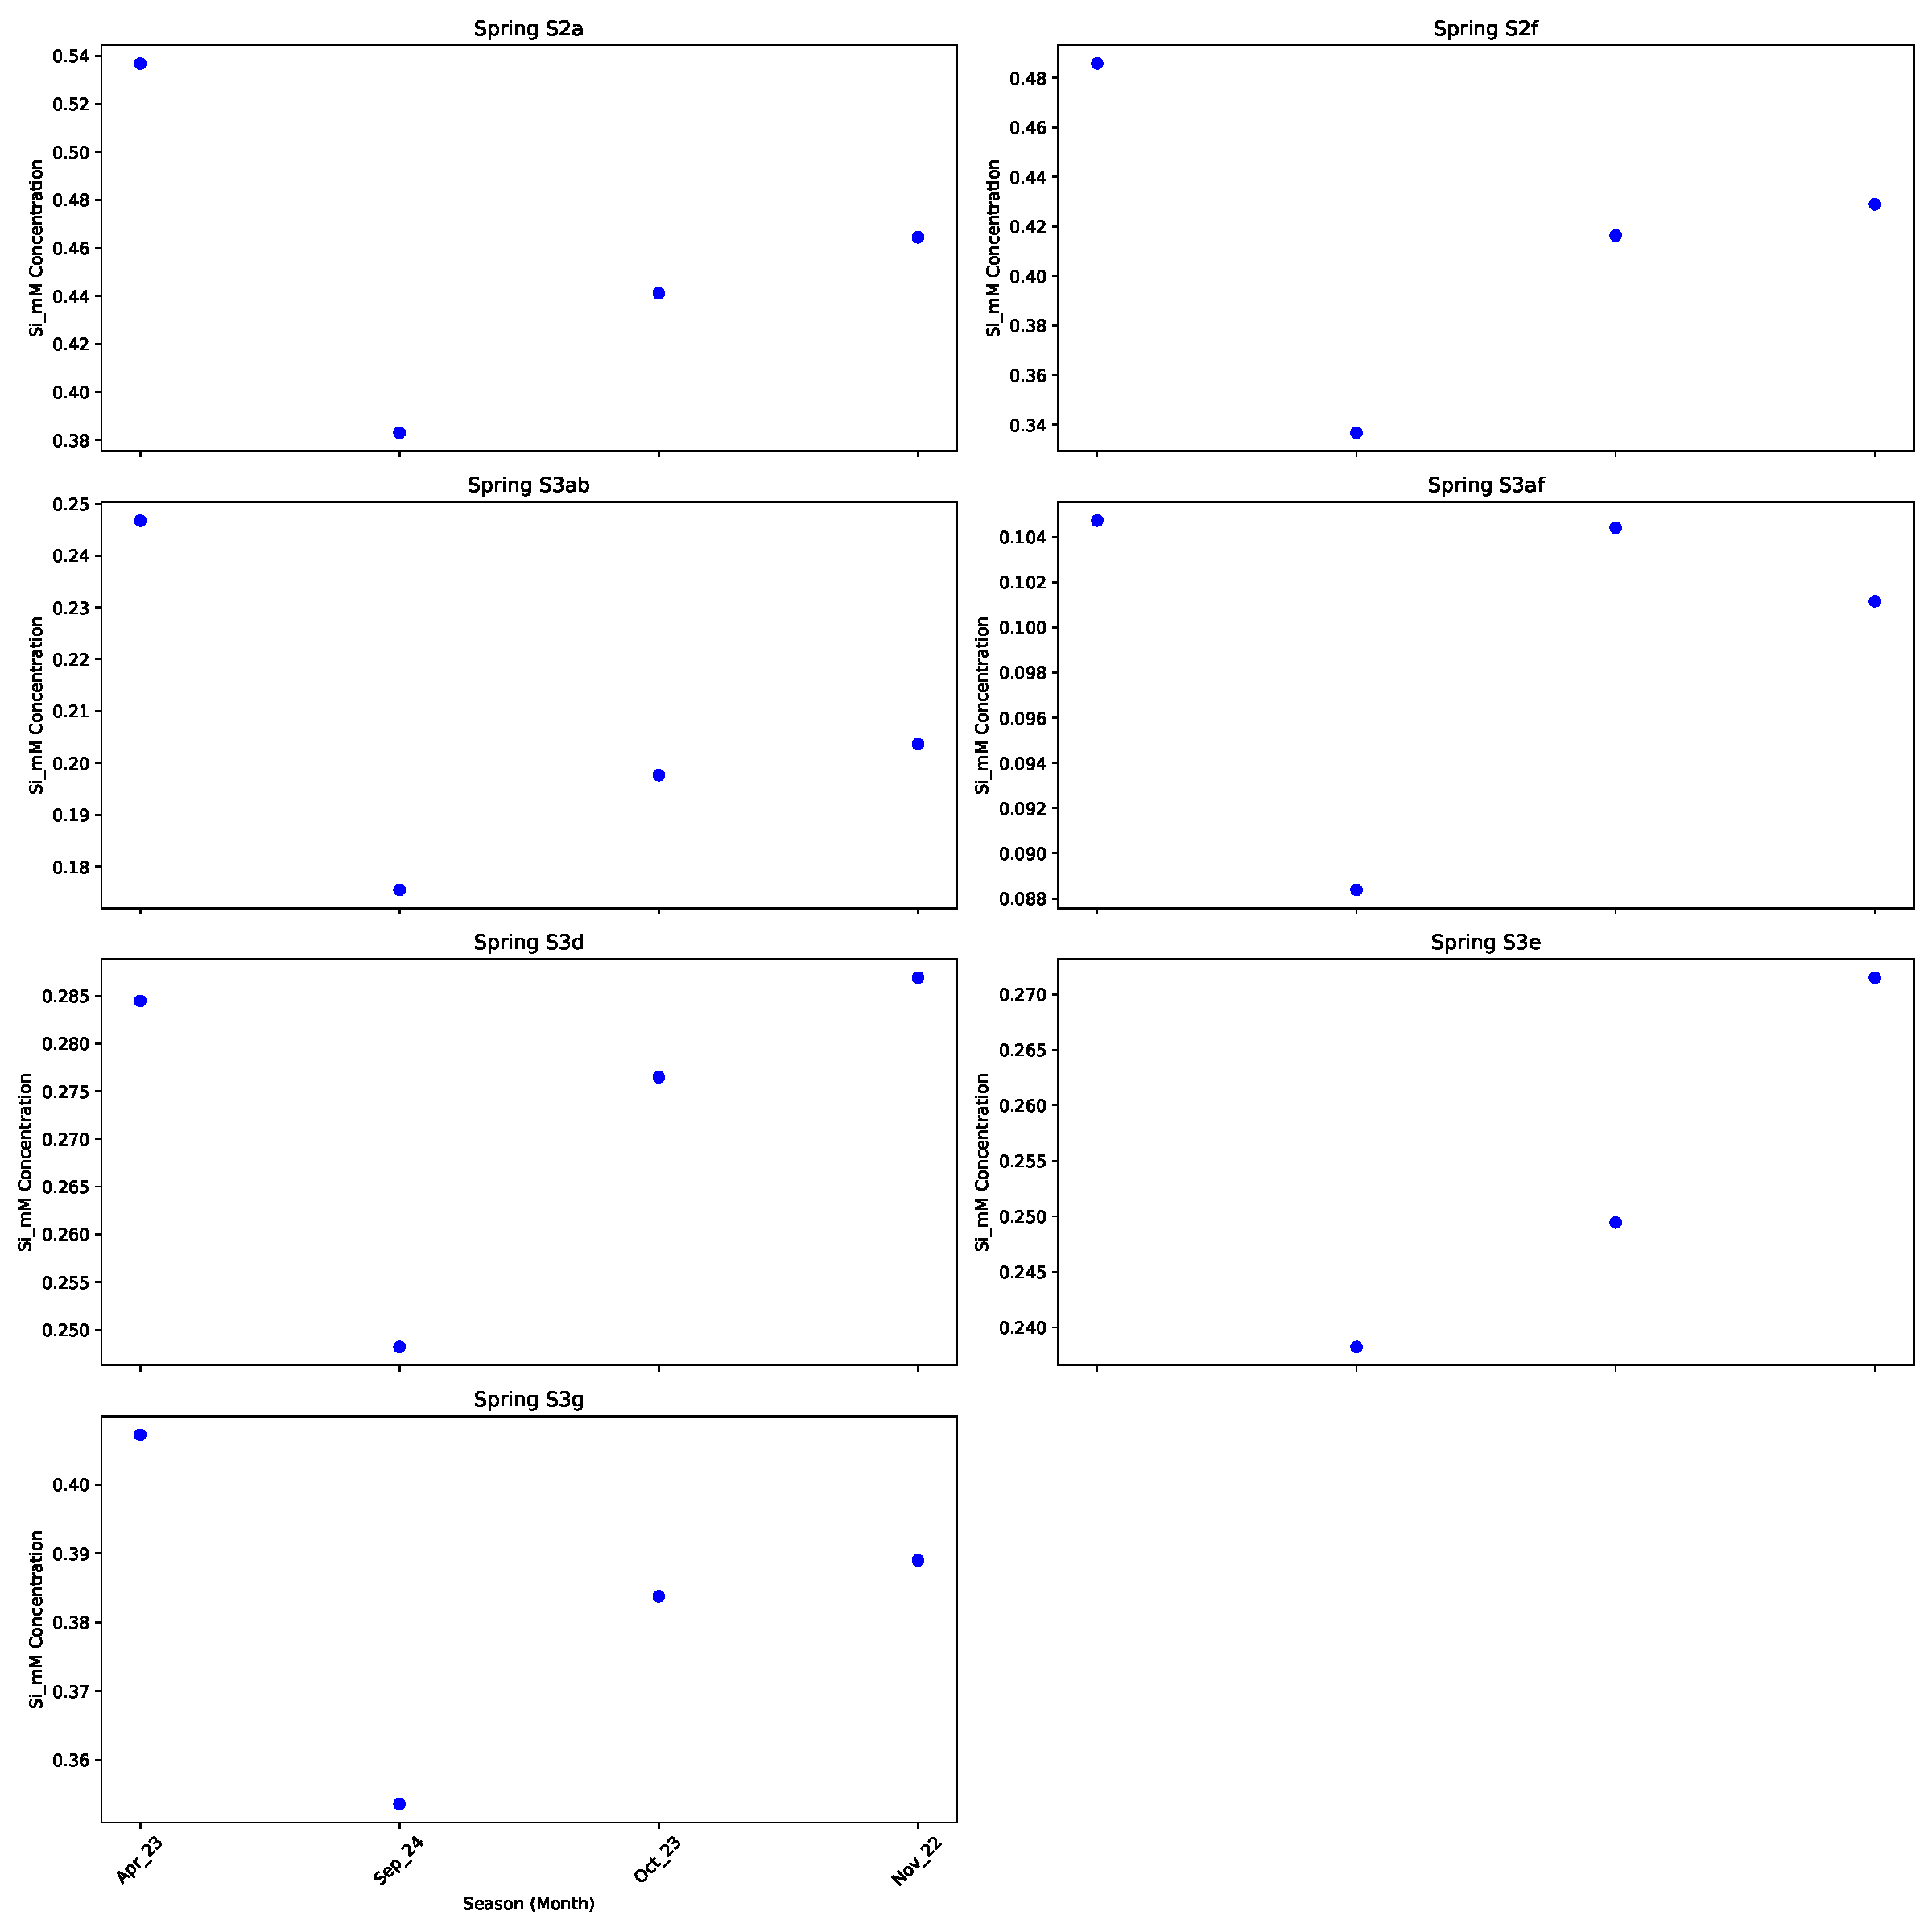
\includegraphics[width=\textwidth]{Si_mM_concentrations_springs.pdf}
    \caption{Seasonal changes in spring concentration indicating monsoonal precipitation influence.}
    \label{fig:seasonal_changes}
\end{figure}

\FloatBarrier


\begin{figure}[h]
    \centering
    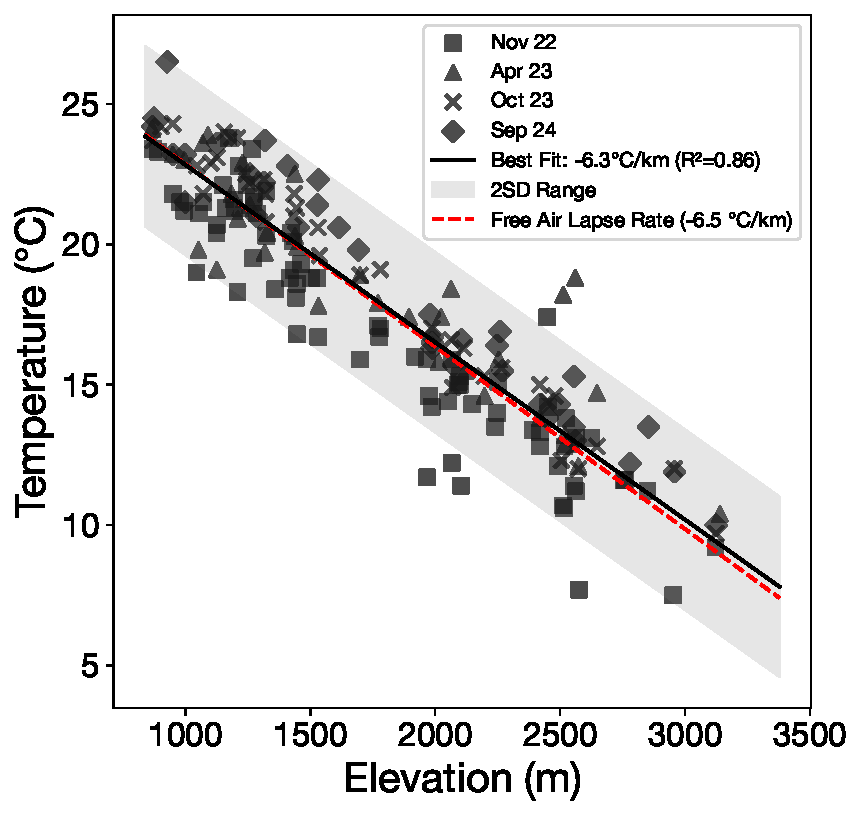
\includegraphics[width=\textwidth]{Temperature_Elevation_Season.pdf}
    \caption{Temperature cahnges}
    \label{fig:seasonal_change2}
\end{figure}

\FloatBarrier


\subsection{Time series spring concentration changing over time}
Concentration increases then decreases with monsoon.

\begin{figure}[h]
    \centering
    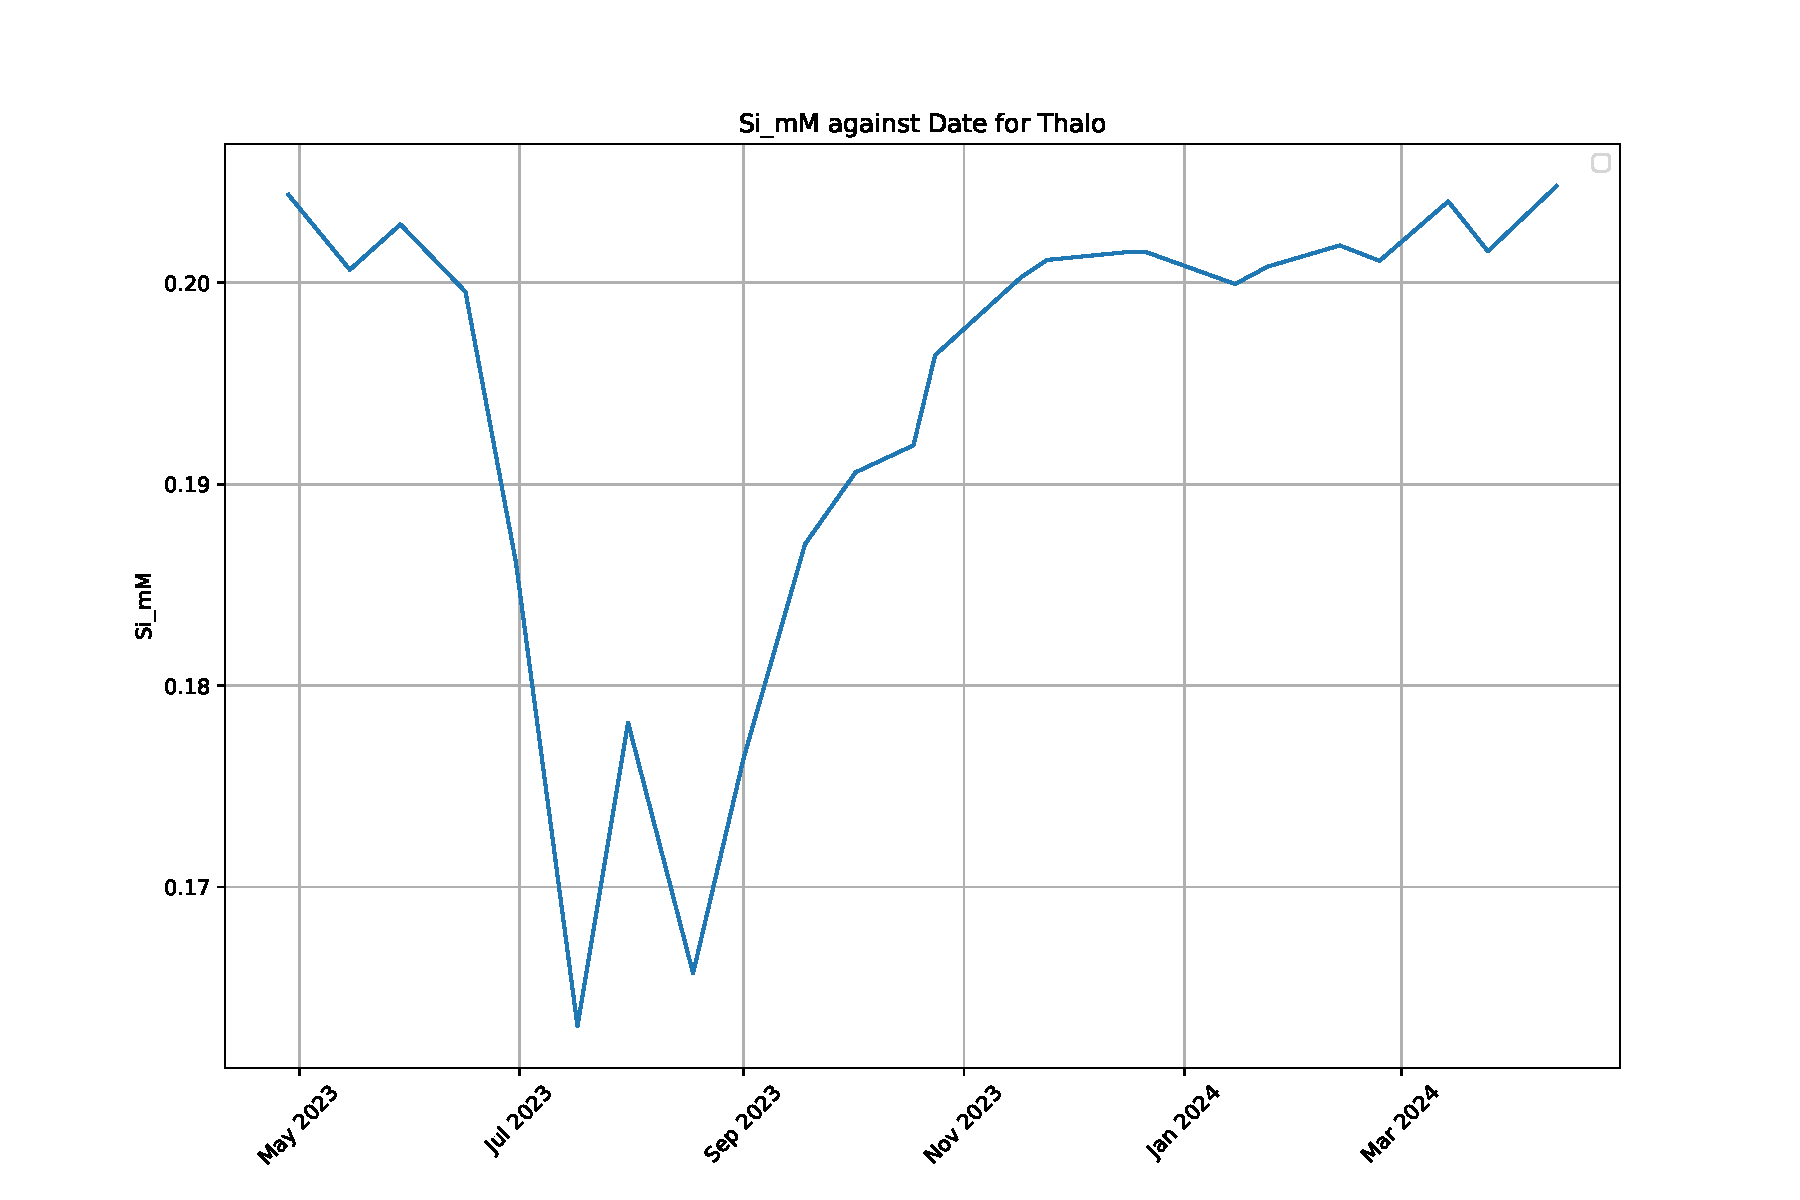
\includegraphics[width=\textwidth]{Si_mM_Thalo_timeseries.pdf}
    \caption{Time series of spring concentration changes over time.}
    \label{fig:time_series_changes}
\end{figure}

\FloatBarrier

\subsection{Spatial concentration changes between the springs}

\begin{figure}[h]
    \centering
    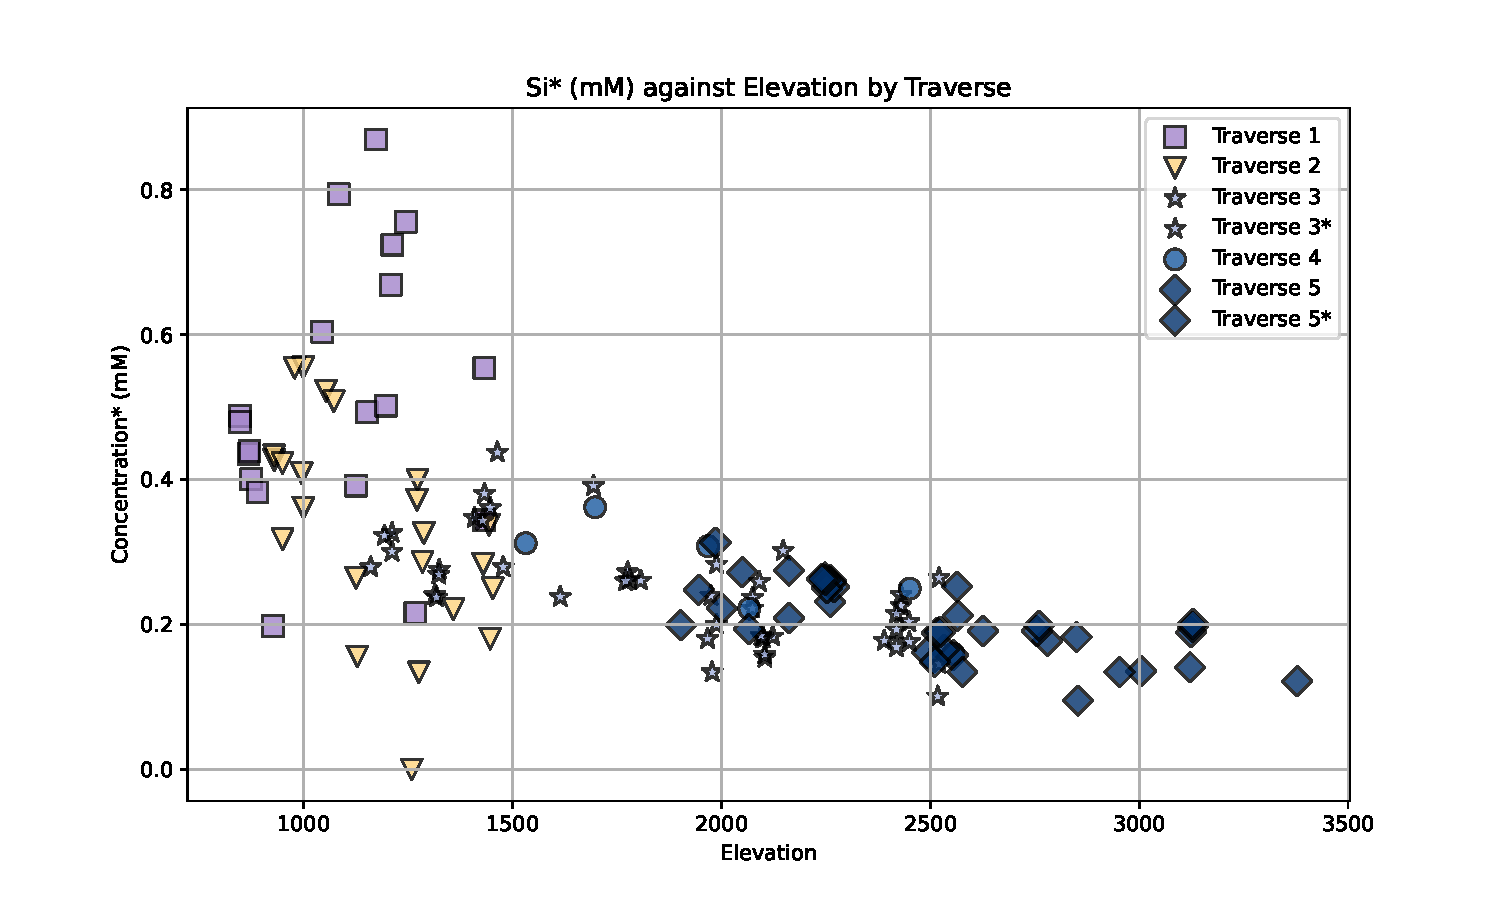
\includegraphics[width=\textwidth]{Si_mM_EC_Elevation.pdf}
    \caption{How Si changes with elevation}
    \label{fig:spatial_changes_spring1}
\end{figure}

\FloatBarrier

\begin{figure}[h]
    \centering
    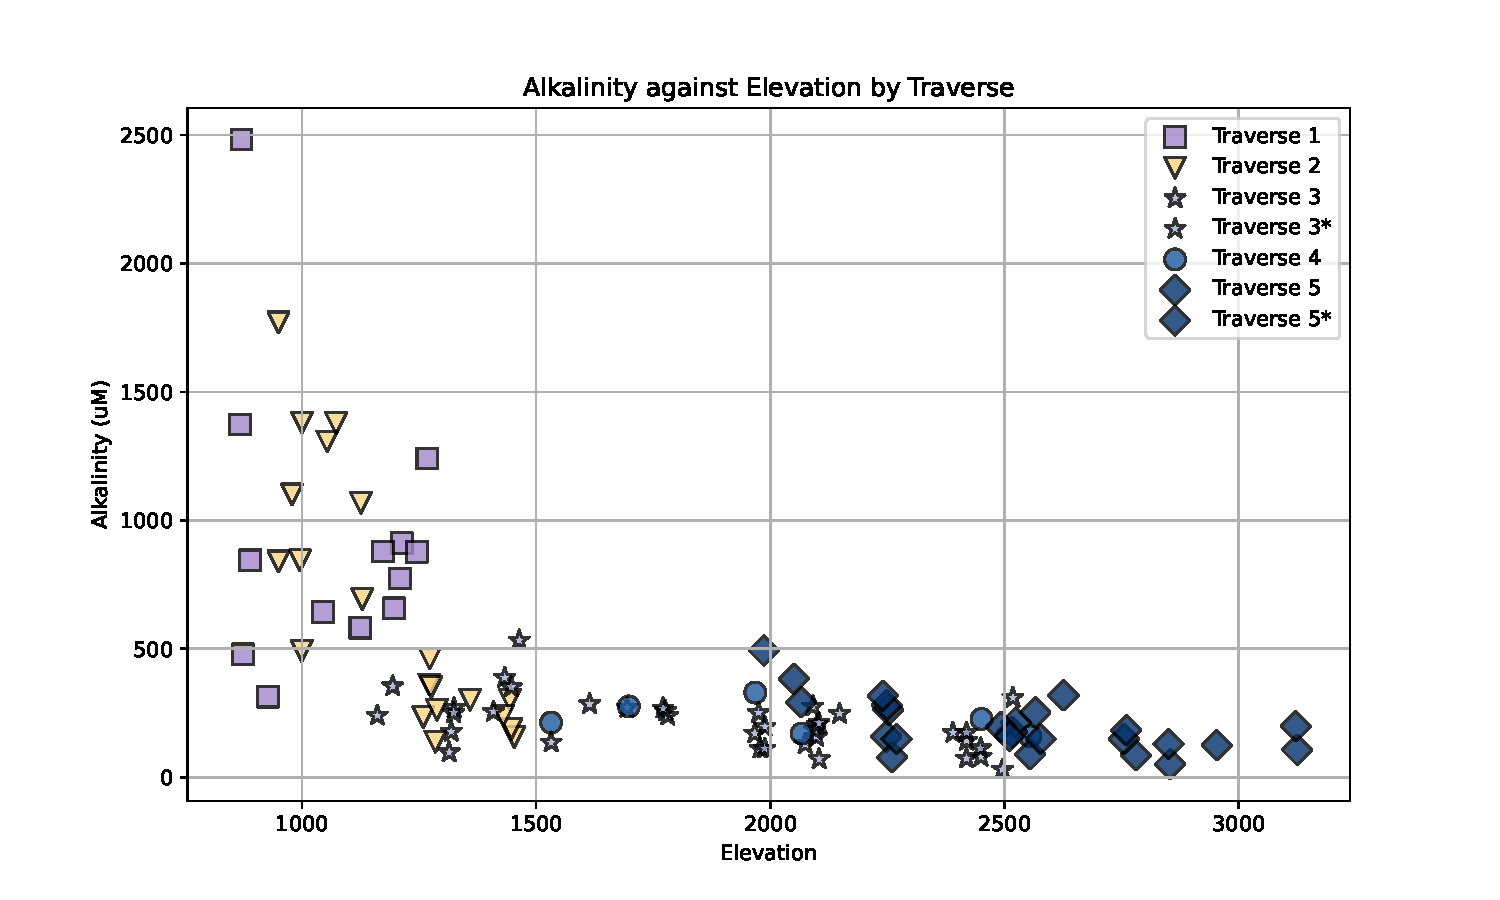
\includegraphics[width=\textwidth]{Alkalinity_Elevation.pdf}
    \caption{How Alkalinity changes with elevation}
    \label{fig:spatial_changes_spring2}
\end{figure}

\FloatBarrier

\begin{figure}[h]
    \centering
    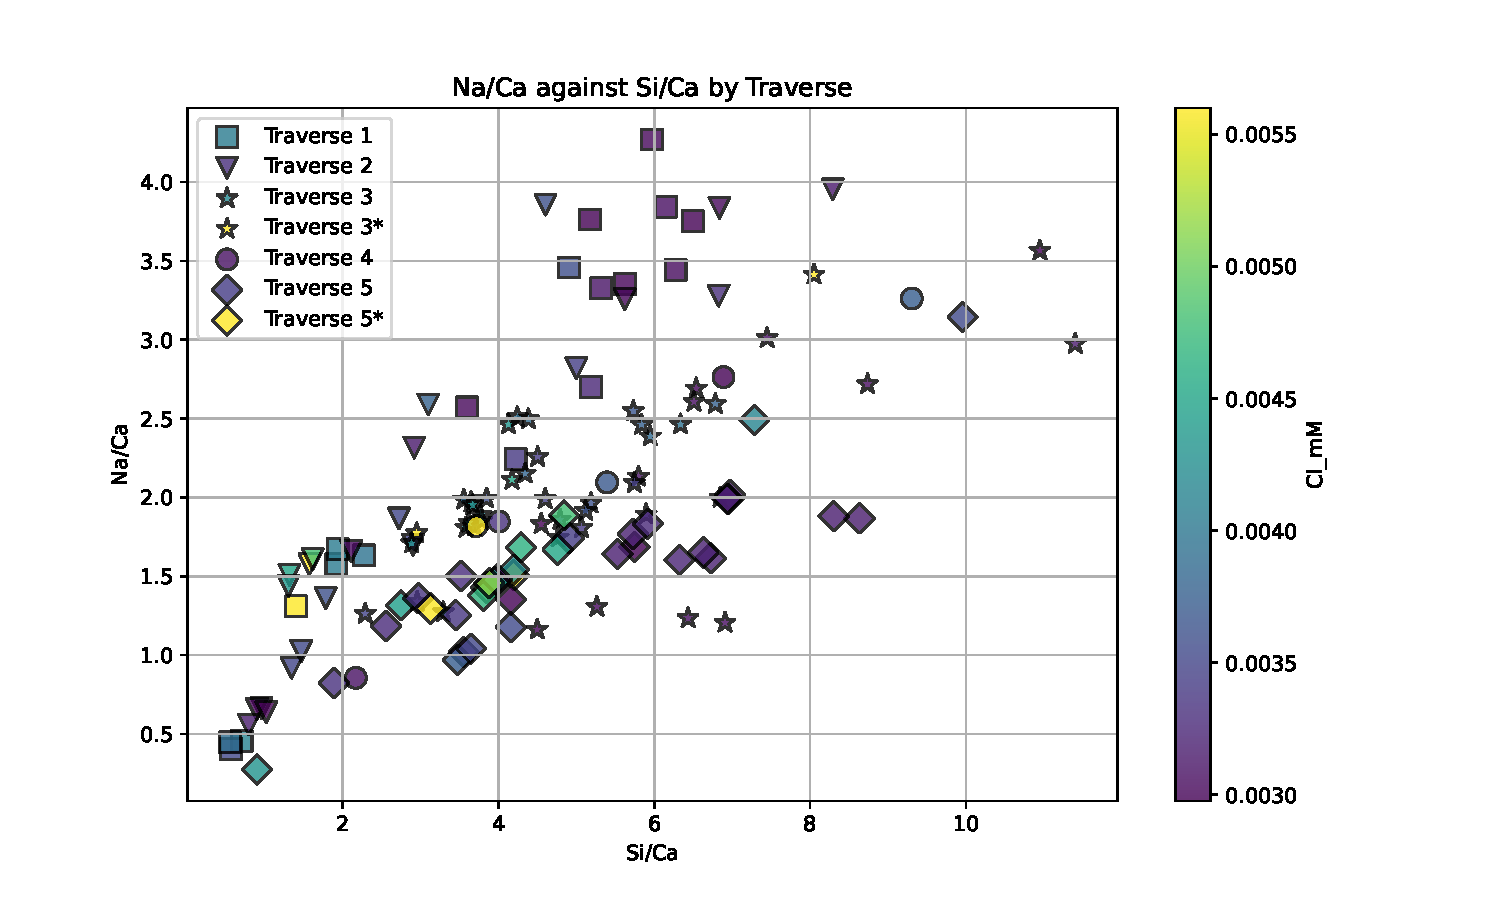
\includegraphics[width=\textwidth]{SiCaNaCa.pdf}
    \caption{Si/Ca against Na/Ca. Clear differences between traverses.}
    \label{fig:spatial_changes_spring3}
\end{figure}

\FloatBarrier

\begin{figure}[h]
    \centering
    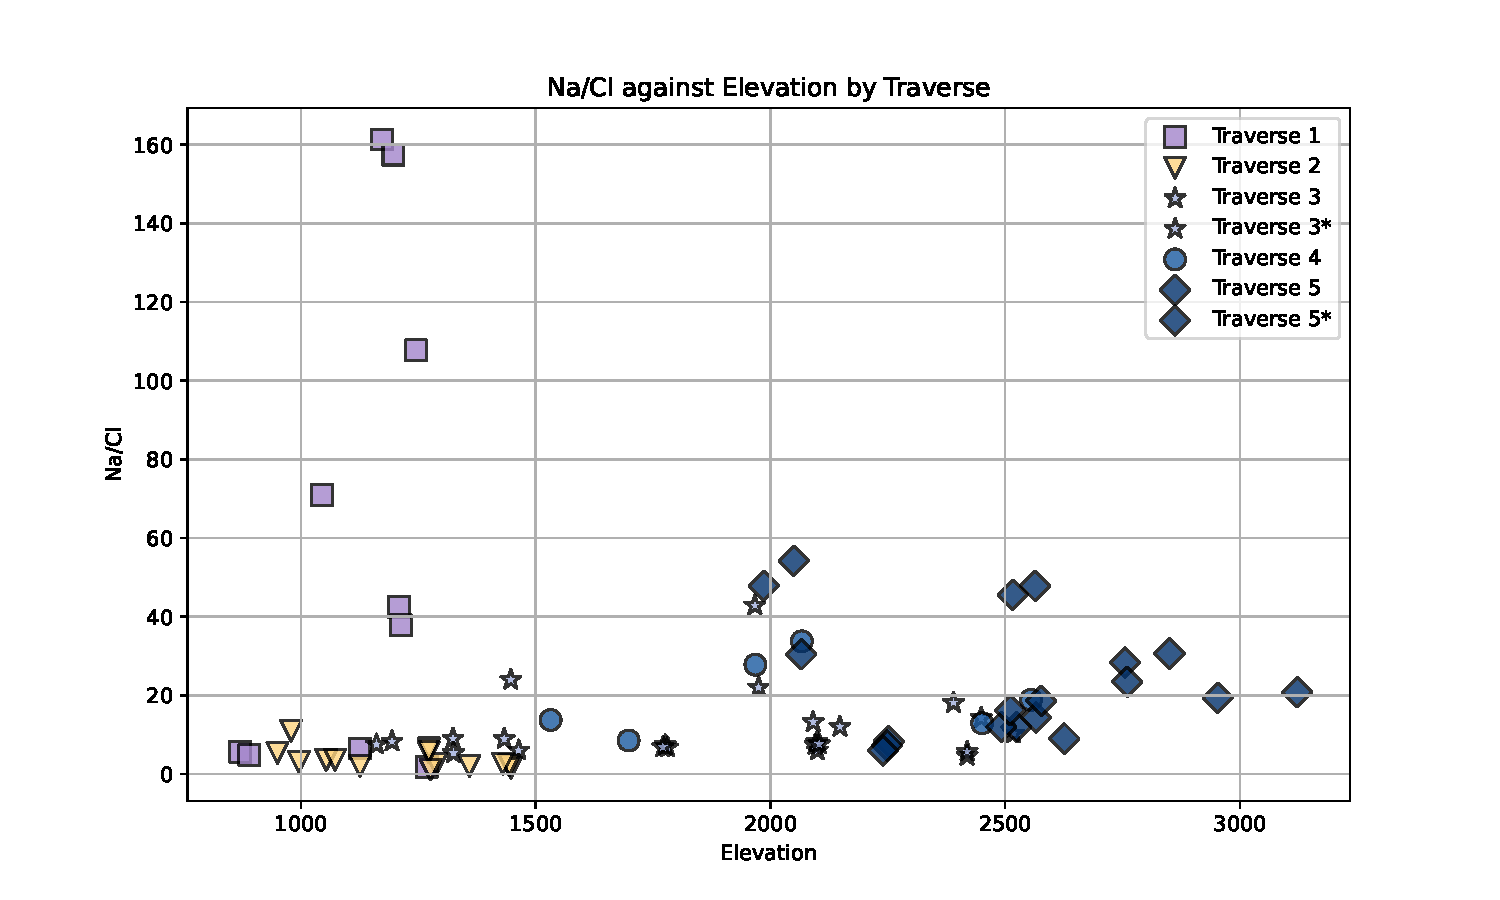
\includegraphics[width=\textwidth]{NaClEl.pdf}
    \caption{NaCl against elevation coloured by traverse -  super low Cl}
    \label{fig:spatial_changes_spring4}
\end{figure}

\FloatBarrier


\begin{figure}[h]
    \centering
    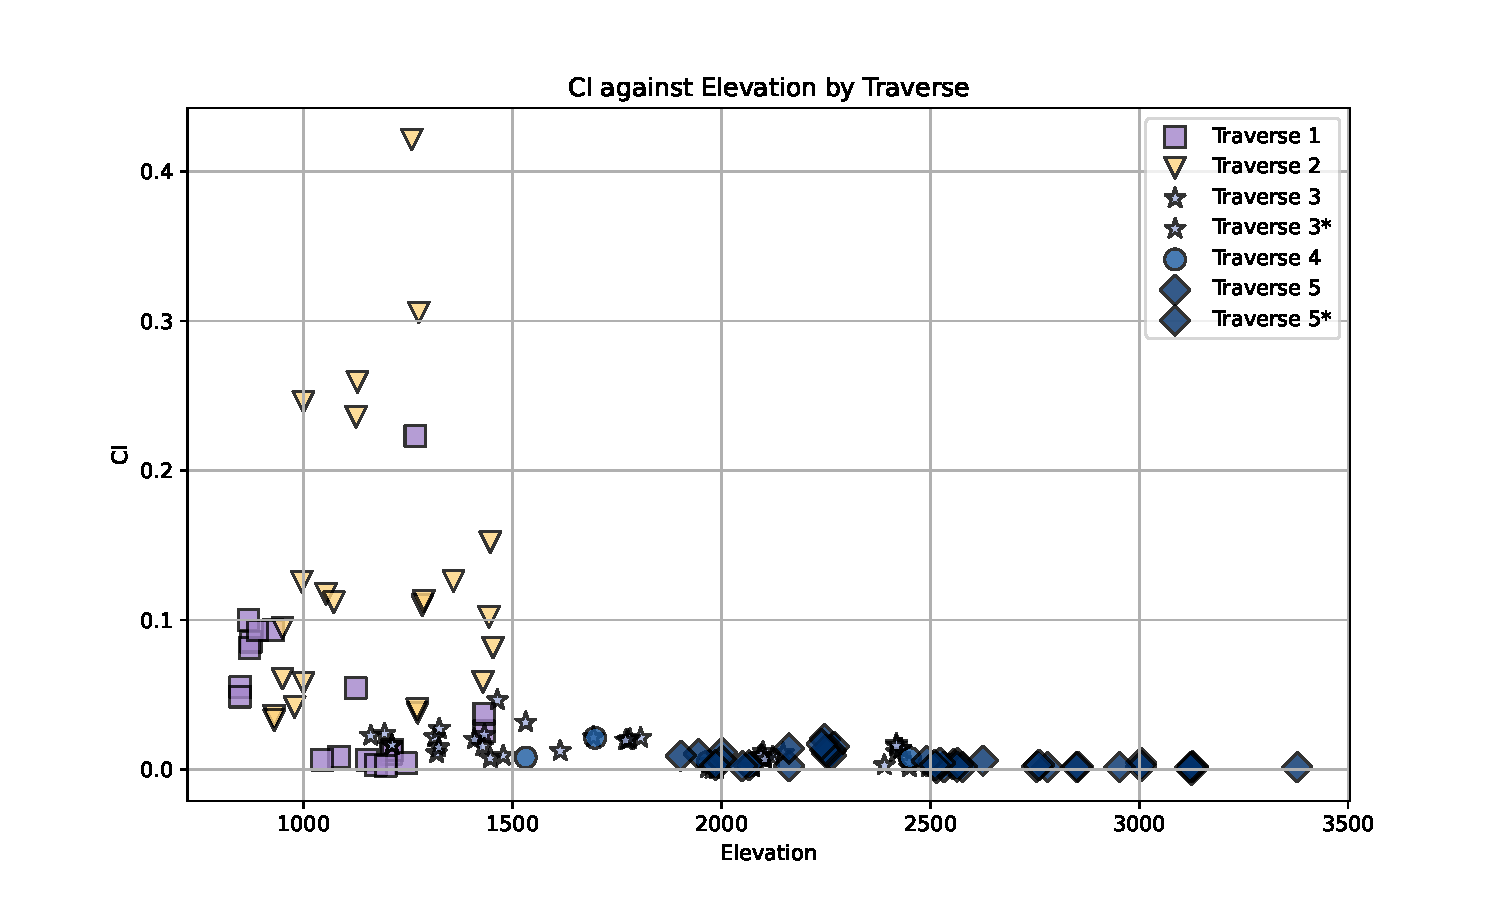
\includegraphics[width=\textwidth]{ClEl.pdf}
    \caption{Cl against elevation coloured by traverse - Potential evaporite influence on traverse 2 water chemistry}
    \label{fig:spatial_changes_spring5}
\end{figure}

\FloatBarrier



\subsection{Sr isotope against 1/Sr data}
To eliminate evaporation, shows the differences between the springs.

\begin{figure}[h]
    \centering
    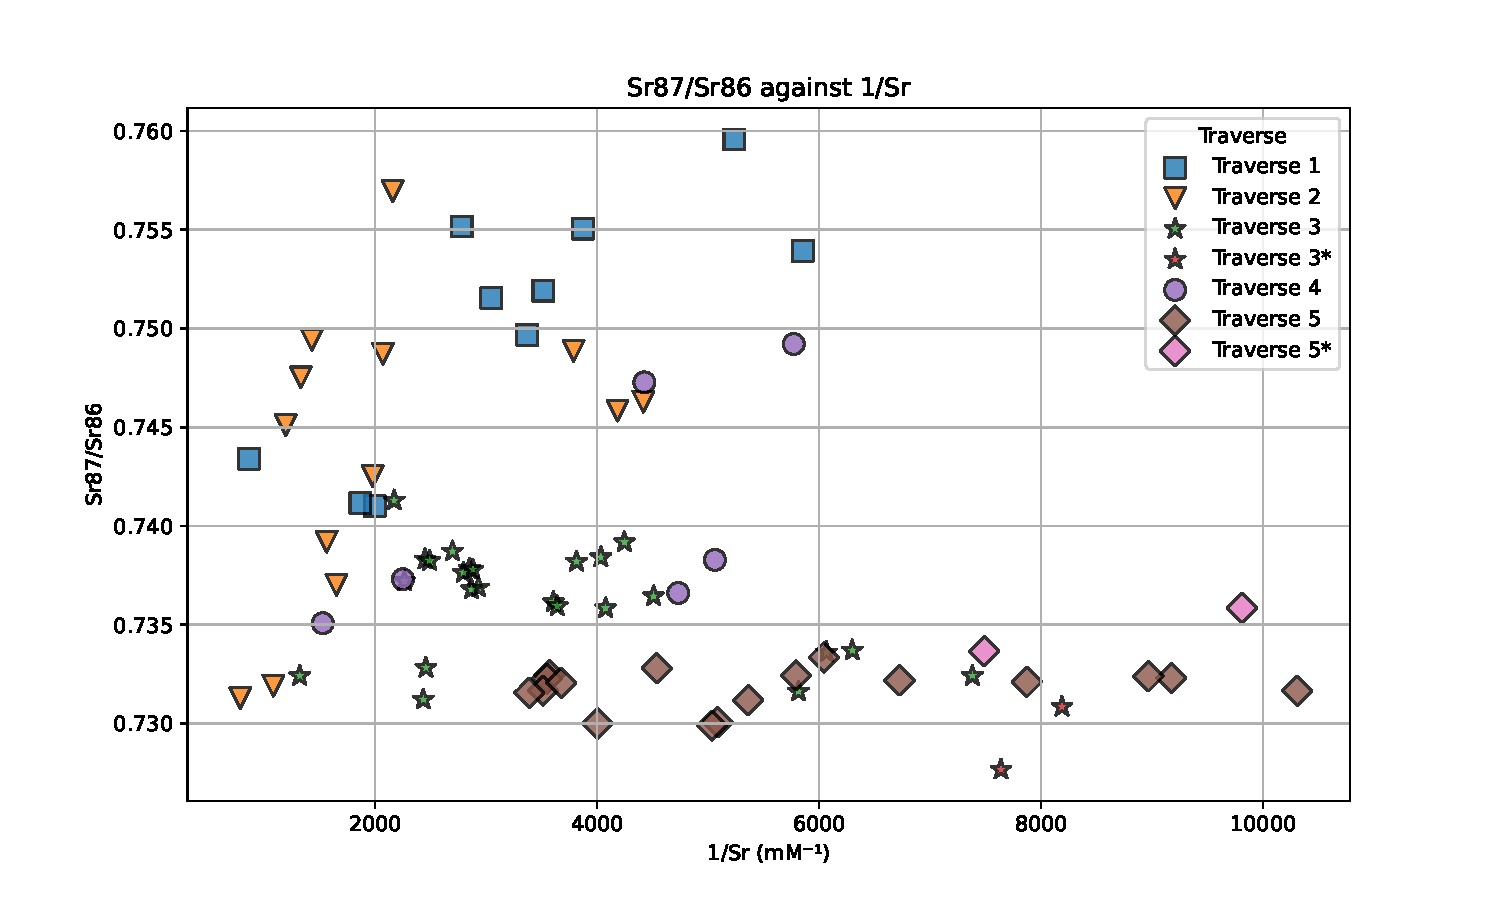
\includegraphics[width=\textwidth]{Sr87_Sr86_1_Sr.pdf}
    \caption{Strontium isotope differences display difference in lithology tapped in. Cite Quade and Tipper papers}
    \label{fig:spatial_changes_spring6}
\end{figure}

\FloatBarrier


\subsection{Traverse 3 is the best sampled and least influenced}
This will be modelled.

\begin{figure}[h]
    \centering
    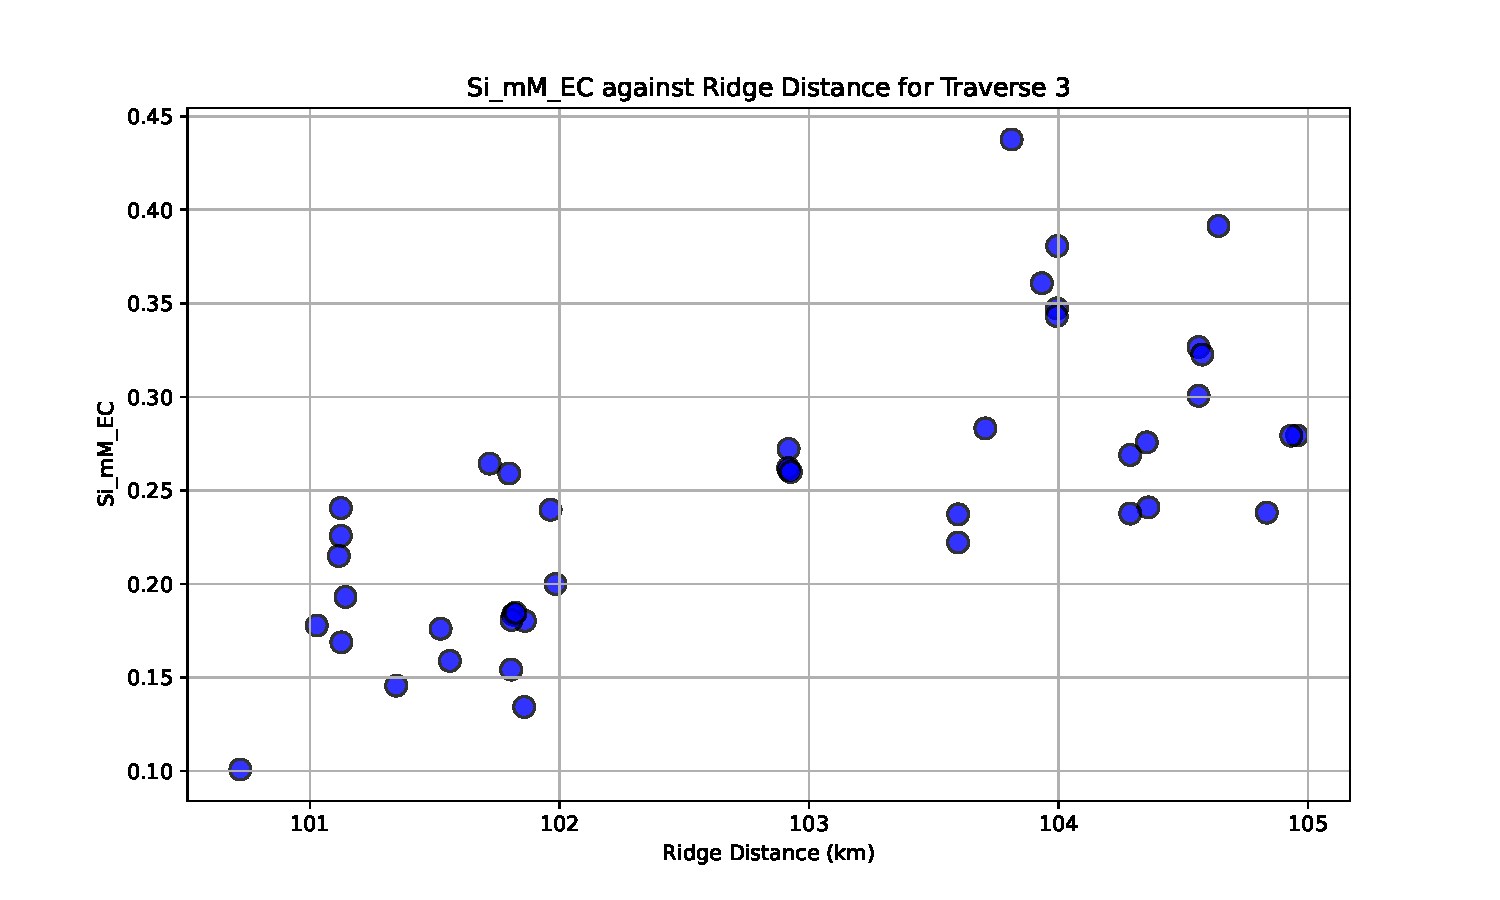
\includegraphics[width=\textwidth]{Si_mM_EC_Ridge_Distance.pdf}
    \caption{How Si varies for Traverse 3, and showing the wide variety of samples}
    \label{fig:spatial_changes_spring7}
\end{figure}

\FloatBarrier

\begin{figure}[h]
    \centering
    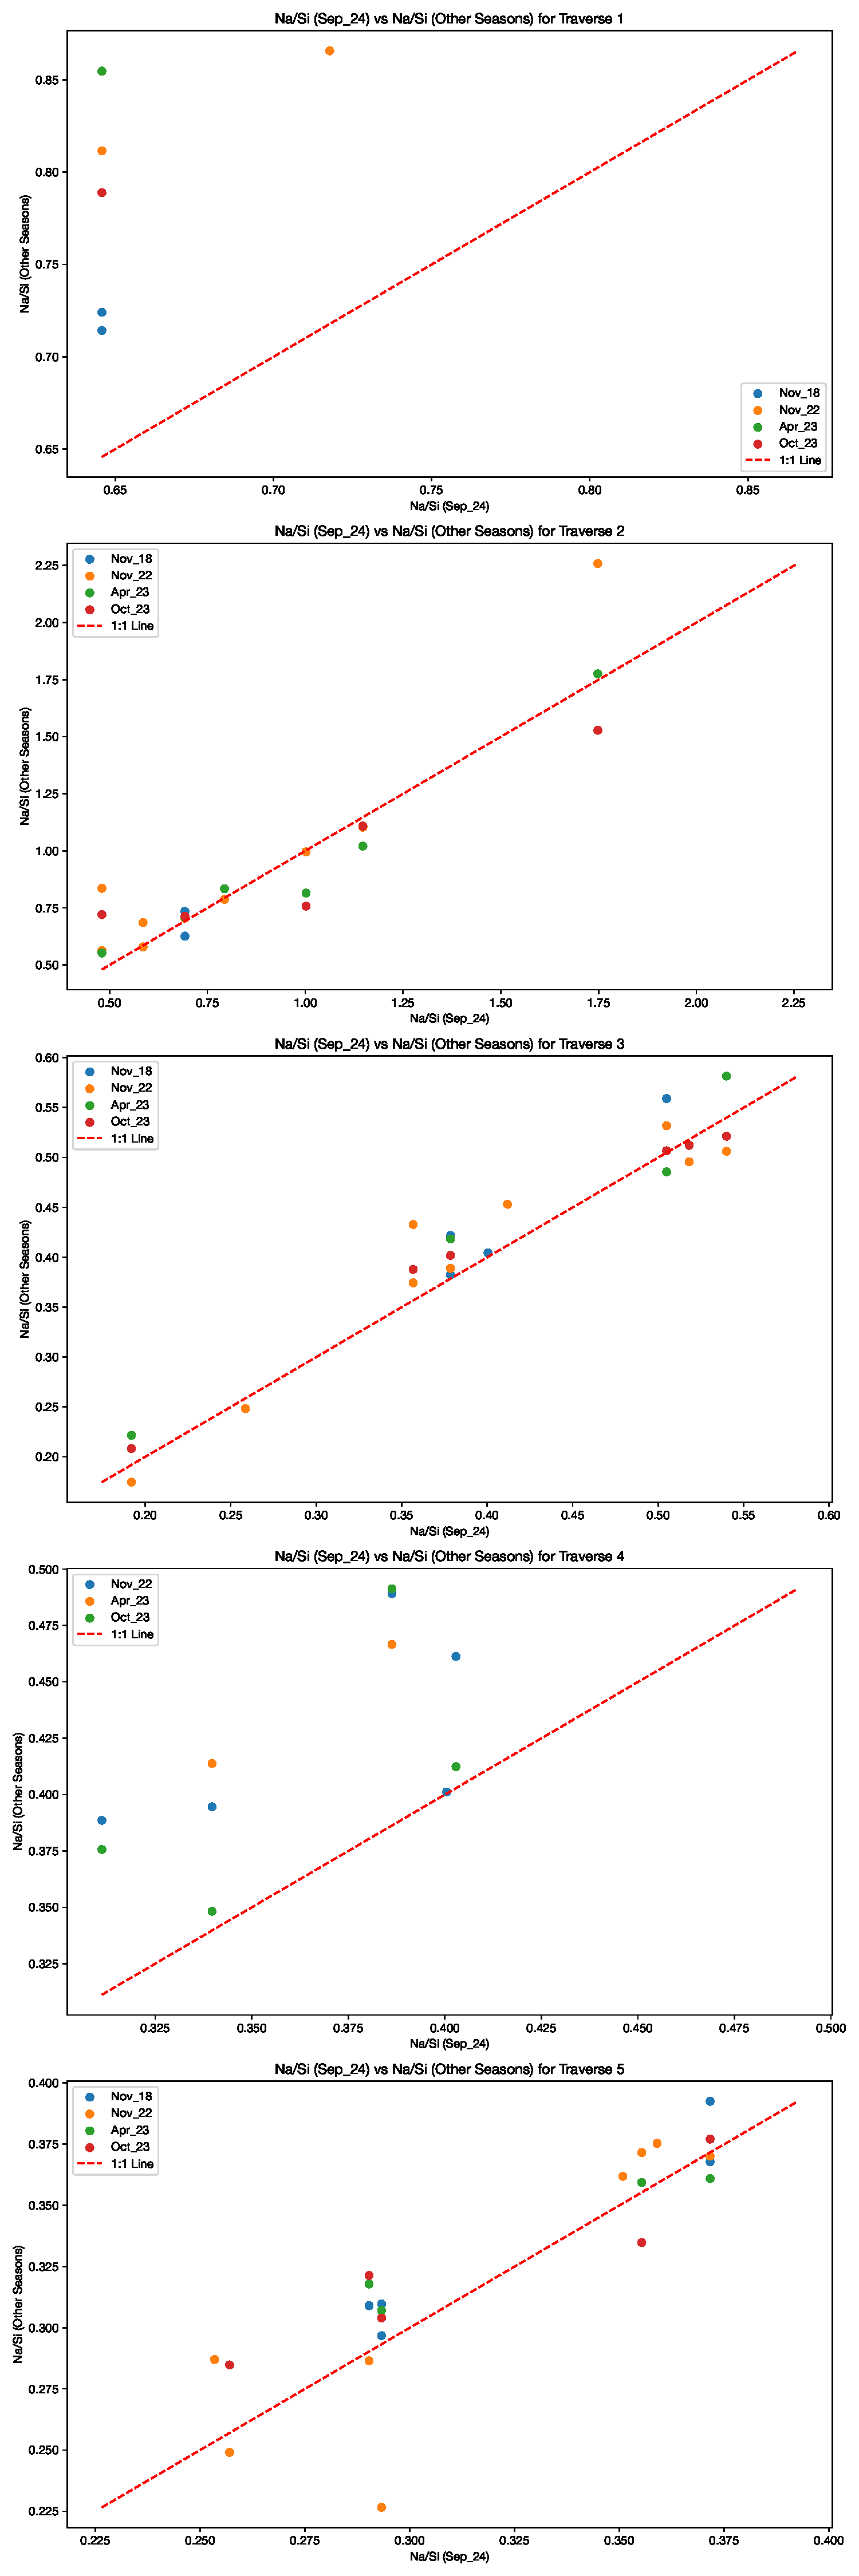
\includegraphics[width=0.5\textwidth]{Na_Si_AllTrav.pdf}
    \caption{Na/Si for all traverses, Traverse 3 is pretty neat}
    \label{fig:spatial_changes_spring8}
\end{figure}

\FloatBarrier


\begin{figure}[h]
    \centering
    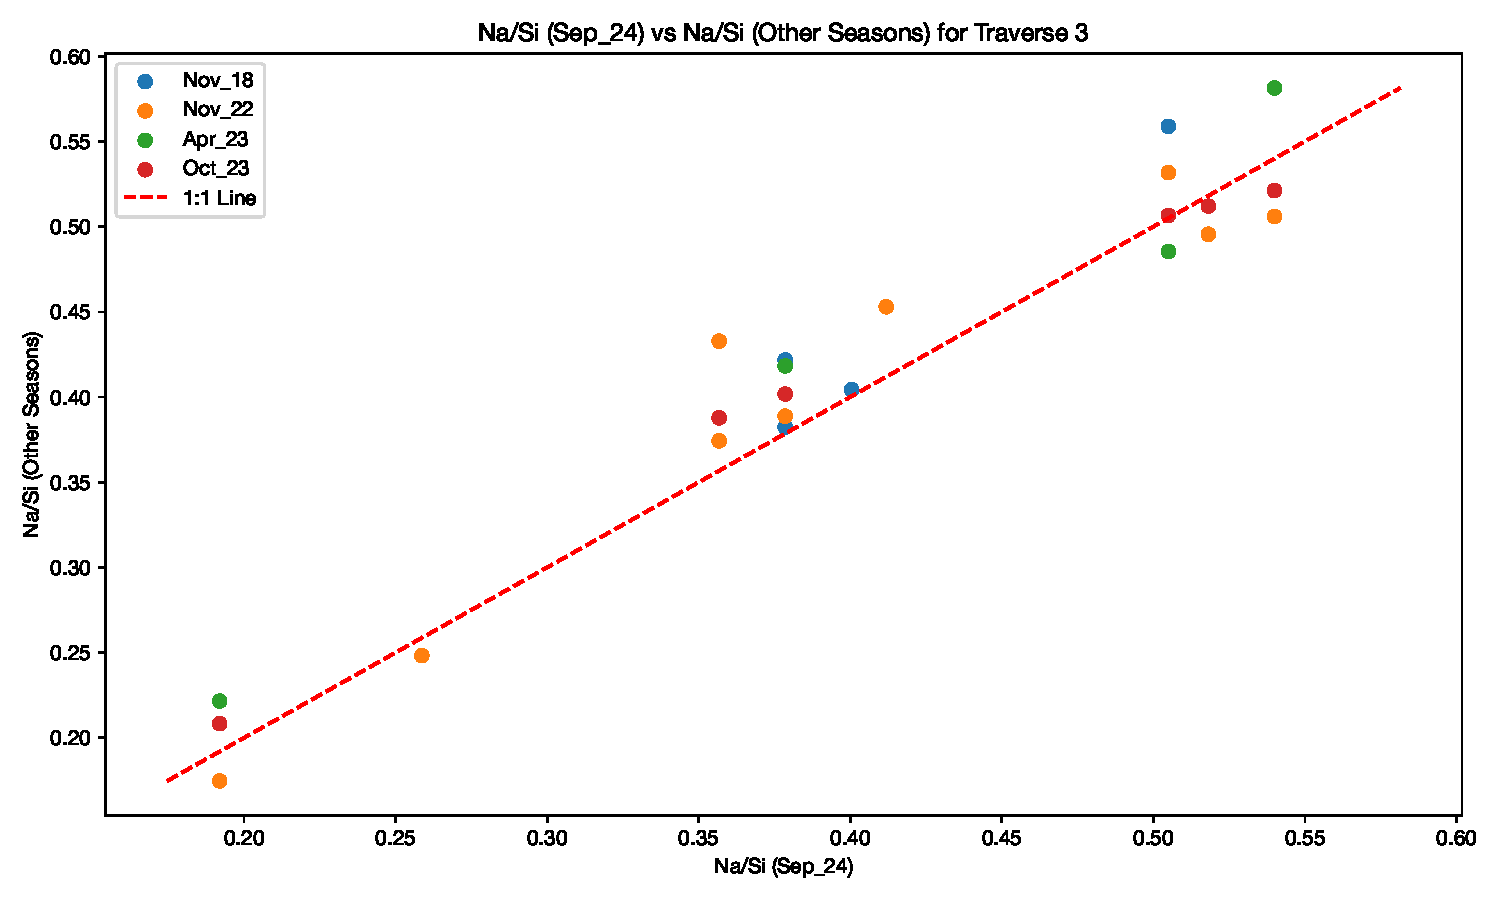
\includegraphics[width=\textwidth]{Na_Si_Trav3.pdf}
    \caption{Na/Si for Traverse 3 is pretty neat}
    \label{fig:spatial_changes_spring9}
\end{figure}

\FloatBarrier

\begin{figure}[h]
    \centering
    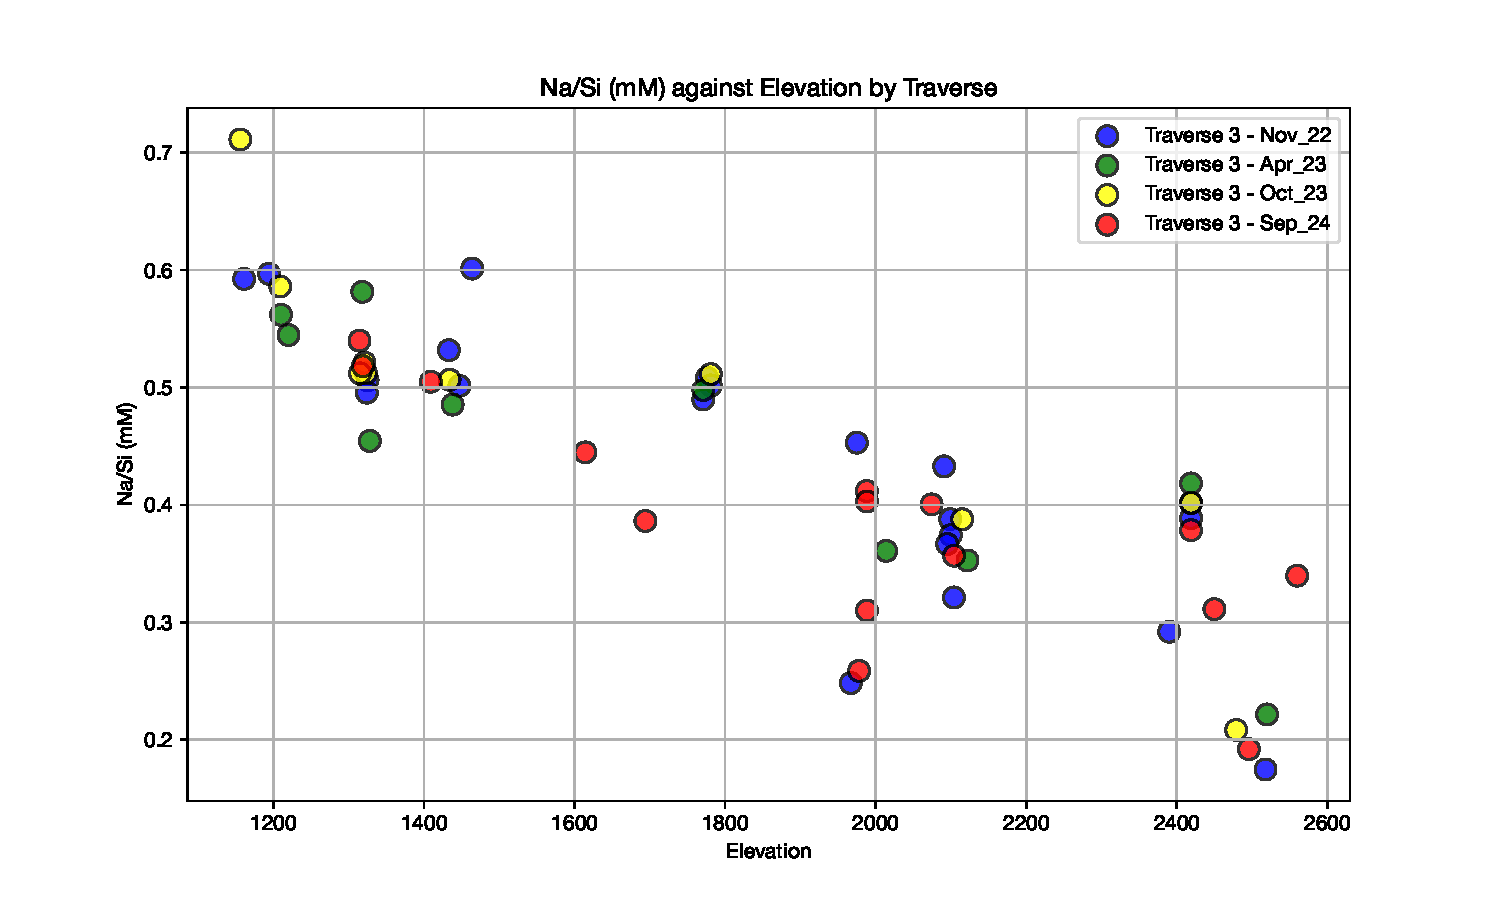
\includegraphics[width=\textwidth]{Na_Si_Elevation.pdf}
    \caption{Na/Si for Traverse 3 is pretty neat. Consistently sampled flow paths}
    \label{fig:spatial_changes_spring10}
\end{figure}

\FloatBarrier


